%%%%%%%%%%%%%%%%%%%%%%%%%%%%%%%%%%%%%%%%%%%%%%%%%%%%%%%
% Please note that whilst this template provides a 
% preview of the typeset manuscript for submission, it 
% will not necessarily be the final publication layout.
%
% letterpaper/a4paper: US/UK paper size toggle
% num-refs/alpha-refs: numeric/author-year citation and bibliography toggle

%\documentclass[letterpaper]{aejstyles}
\documentclass[a4paper,alpha-refs]{eSpectra}

%%% Journal toggle; only specific options recognised.
\journal{aej}

\usepackage{graphicx}
\usepackage{siunitx}
\usepackage[spanish]{babel}             % Spanish for default (Abstract. References, Appendix, tables, and figures names).

\usepackage{comment} 
%\setcounter{page}{24}
 
%\usepackage[left]{lineno}
%\linenumbers

%%% Flushend: You can add this package to automatically balance the final page, but if things go awry (e.g. section contents appearing out-of-order or entire blocks or paragraphs are coloured), remove it!
% \usepackage{flushend}

\title{Variabilidad atmosf\'erica en Marte y la Tierra inducidas por la actividad solar}

%%% Use the \authfn to add symbols for additional footnotes, if any. 1 is reserved for correspondence emails; then continuing with 2 etc for contributions.
\author[1,\authfn{1},]{Johan Nicolás Molina Córdoba}
\author[1]{Santiago Vargas Domínguez}
\author[2]{Jorge Ivan Zuluaga Callejas}

\affil[1]{Observatorio Astronómico Nacional, Universidad Nacional de Colombia, Bogotá D.C., Colombia}
\affil[2]{Instituto de Física, Universidad de Antioquia, Medellín, Colombia}

%%% Author Notes
\authnote{\authfn{1}Estudiante de Maestría en Ciencias - Astronomía (jomolinac@unal.edu.co)}


%%% Paper category: Other categories include: Research Article, Review, News, Announcements, Interviews, Opinion, Resources & Activities, Book Review, Correspondences, Best practice,
\papercat{Artículo Científico}

%%% "Short" author for running page header
\runningauthor{First et al.}

%%% Should only be set by an editor
\jvolume{1}
\jnumber{1}
\jyear{2023}
\begin{document}
\begin{frontmatter}
\maketitle
\begin{abstract}
En este trabajo se presentan resultados preliminares del estudio de correlaci\'on entre atm\'osferas planetarias (Tierra y Marte) y flujo energ\'etico solar en radio a $\lambda = 10.7$ cm. En particular, se esbozan resultados de an\'alisis  de \textit{proxies} que permiten hacer estimaciones de la densidad de agua atmosf\'erica en las diferentes capas de la atm\'osfera intermedia y baja de Marte. Para el caso de la Tierra se emplea información del \textit{National Oceanic and Atmospheric Administration} (NOAA) a trav\'es del modelo emp\'irico NRLMSISE 00, donde se obtienen datos de abundancias de N$_2$, O$_2$,N, H$_2$, Ar y He en una ventana temporal de 1961-2021 a 55 y 105 km de altura.  Para la caracterizaci\'on de la variabilidad en la atm\'osfera marciana se toman datos registrados por el instrumento SPICAM de la sonda \textit{Mars Express} en una ventana de tiempo de 2004-2018. Los datos de flujo solar son obtenidos tambi\'en del modelo emp\'irico NRLMSISE 00. La propuesta se consolida en el \'ambito de las ciencias planetarias, que involucra el clima espacial y las condiciones astrobiol\'ogicas en el entorno solar, dando esbozos sobre la importancia de contemplar la b\'usqueda de modelos climatol\'ogicos a escala del Sistema Solar, que den cuenta de conexiones y sinergias entre los cambios que experimentan los planetas asociados a la variabilidad solar durante el ciclo de actividad de la estrella. Los resultados manifestan la existencia de correlación entre grados de concentración de diferentes especies químicas de las atmósferas para los dos sistemas planetarios estudiados  y la señal de flujo solar. %
\end{abstract}

\begin{keywords}
Atmósferas Planetarias; Marte; Ciclo Solar; Modelos Climatológicos; NRLMSISE 00; Clima Espacial. 
\end{keywords}
\end{frontmatter}

\section{Introducción}

En el contexto de estudio de las atm\'osferas planetarias, el env\'io de sondas espaciales orbitales en las atm\'osferas de distintos planetas del sistema solar (incluida la Tierra) desde la d\'ecada de 1960, ha sido fundamental para reconocer la variabilidad atmosf\'erica asociada a diferentes fen\'omenos, por ejemplo, ciclos estacionales \citep{Mars_seasonal_2002}, actividad magn\'etica, o estados de ionizaci\'on en la ionosfera producidos por la incidencia de la radiaci\'on UV proveniente del Sol \citep{Tian_2022}. En el marco de estudio de la caracterizaci\'on atmosf\'erica de un planeta, su composici\'on qu\'imica es un aspecto de especial inter\'es en la investigaci\'on, tanto como insumo de conocimiento para estudiar posibles condiciones de habitabilidad o posibles proxies que determinan si en alg\'un momento dado, un planeta fue habitable.

De los modelos conocidos actualmente en el estudio de Marte, se identifica que al igual que como ocurre en la Tierra, la atm\'osfera superior marciana se ioniza principalmente por la incidencia de radiaci\'on UV proveniente del Sol \citep{Tian_2022}, y la ionosfera se constituye de picos de densidad electr\'onica a lo largo de 120 km de columna vertical exterior de la atm\'osfera marciana \citep{Mars_ionosf_2011}. En los perfiles espaciales y temporales hay varios niveles donde coexiste la atmósfera neutra con iones de diferentes especies químicas. Por otro lado, Marte tiene una regi\'on bien mezclada de la homosfera con la homopausa a 120 km de altitud. la termosfera se define como la regi\'on por encima de la cual los gases se separan difusivamente con especies qu\'imicas individuales, siguiendo sus alturas de escala. Finalmente esta regi\'on se fusiona con la exosfera, donde los gases m\'as livianos pueden energizarse para alcanzar velocidades de escape. Por lo general, este proceso de p\'erdida comienza alrededor de los 220 km de altura llamado exobase, donde las alturas de escala y los caminos libres medios son comparables. La din\'amica de esta regi\'on est\'a impulsada por los flujos de energ\'ia y momento rotacional de los planetas, además de las ondas de marea que se propagan a trav\'es de la atm\'osfera inferior \citep{kamsali_2021}. Por efectos de la radiaci\'on solar ultravioleta extrema (EUV), en la atm\'osfera inferior se introducen part\'iculas energ\'eticas inducidas por llamaradas y plasma de viento solar de flujo variable \citep{petrosyan_mars_2011}.

En general, se han encontrado con diferentes grados de abundancia, diversas especies qu\'imicas como Ar, H, O, N, CO$_2$ y H$_2$O en Marte \citep{Mars_ab_2017, Mars_ab_2014, economou_2008}. Estas diferentes especies caracterizan la composici\'on de las atm\'osferas tanto de la Tierra como de Marte, que var\'ian, seg\'un lo conocido, de acuerdo con periodos estacionales relacionados con el movimiento orbital de estos dos cuerpos celestes. 

Entre las sondas caracter\'isticas que han rastreado la atm\'osfera de Marte, la misi\'on de exploraci\'on \textit{Mars Express} es una de las m\'as antiguas y que a\'un est\'a en funcionamiento \citep{Mars_Express}. Esta acumula un tiempo de almacenamiento de datos que pueden ser procesados para la derivaci\'on de perfiles de densidad de distintas especies qu\'imicas en la atm\'osfera de Marte equivalente a 18 a\~nos. En esta investigaci\'on se retoman datos derivados en el trabajo de \cite{spicam_fedorova_H2O_2021}. Estos son datos de abundancias de vapor de agua, reproducidos a partir de im\'agenes espectrosc\'opicas obtenidas a trav\'es del canal infrarrojo del instrumento cient\'ifico incorporado en \textit{Mars Express}, SPICAM (\textit{Ultraviolet and Infrared Atmospheric Spectrometer}) por el m\'etodo de ocultaci\'on estelar. Esta t\'ecnica consiste en la determinaci\'on de la transmisi\'on atmosf\'erica de la luz proveniente de una estrella, a varias altitudes sobre la superficie de un planeta \citep{estelar_ocult_2006}.

Para los resultados de correlaci\'on de esta entrega preliminar de la investigaci\'on se analizaron en el caso de Marte, perfiles de abundancias y densidades de vapor de agua con datos procesados de SPICAM de \textit{Mars Express}. Y en el caso de la Tierra, perfiles de densidad y abundancia qu\'imica de distintas especies que componen la atm\'osfera. Las especies qu\'imicas analizadas fueron: Ar, N$_2$, O$_2$ y He. Las variabilidades asociadas a estas especies en la atm\'osfera terrestre fueron obtenidas en  el modelo emp\'irico NRLMSISE 00. Este modelo interpola datos a partir de observaciones espectrosc\'opicas llevadas a cabo por la red de sat\'elites GOES (\textit{Geostationary Satellite Server}), que miden abundancias de part\'iculas neutras e ionizadas mediante t\'ecnicas de ocultaci\'on estelar \citep{estelar_ocult_2006}. Los datos de diferentes especies qu\'imicas de la atm\'osfera terrestre son contrastados con datos de flujo solar caracter\'istico F 10.7 cm para buscar posibles correlaciones asociadas a la din\'amica peri\'odica del ciclo solar. 

La din\'amica peri\'odica del Sol ha sido objeto de estudio dentro del campo conocido como astrof\'isica solar. Actualmente se estima que el ciclo asociado a la variabilidad en su actividad dura
alrededor de 11 a\'nos. Este comportamiento c\'iclico se manifiesta en patrones caracter\'isticos de
manchas solares que aparecen en la fotosfera solar, conocidos como patrones de mariposa \citep{Maunder_2021}. Si bien el n\'umero de manchas solares es un indicador de actividad solar, el flujo medido en radio F 10.7 cm es un indicador mas objetivo en cuanto a su detecci\'on y la resoluci\'on asociada a su medici\'on \cite{Lemon_2018}.  

Finalmente, cabe destacar que esta investigaci\'on sigue la misma l\'inea documental (en el contexto del clima espacial y caracterizaci\'on de atm\'osferas planetarias) de trabajos como \cite{kamsali_2021}, en donde se hacen an\'alisis de variabilidad atmosf\'erica a trav\'es de datos de la sonda MAVEN (\textit{Mars Atmosphere and Volatile Evolution}) en dos momentos caracter\'isticos: un máximo y un mínimo solar. Y el trabajo de \cite{Lemon_2018}, en donde se estudia con alta significaci\'on estadística la correlaci\'on entre un evento solar caracter\'istico conocido como terminador (el final de ciclo magn\'etico solar), y las mayores oscilaciones de los \'indices oce\'anicos de la Tierra que determinan los efectos clim\'aticos transitorios: fen\'omenos del ni\~no y la ni\~na.

\section{Observaciones y reducción de datos}

De todos los equipos de experimentos a bordo del orbitador de \textit{Mars Express}, el SPICAM (\textit{Spectroscopy for the Investigation of Characteristics of the Atmosphere of Mars}) es el que lleva a cabo sondeos atmosf\'ericos a trav\'es de t\'ecnicas de ocultaci\'on estelar. Los datos directos son im\'agenes espectrosc\'opicas obtenidas en dos canales diferentes, uno UV y el otro IF. El canal IF analiza datos de absorci\'on relacionados con las abundancias de mol\'eculas de agua, cuya variabilidad es el centro del an\'alisis de los resultados preliminares que fundamentan este documento.

El instrumento equipado en SPICAM en el canal infrarrojo est\'a compuesto por una lente de entrada, un AOTF y dos detectores de un solo p\'ixel, y tiene una resoluci\'on espectral de  $0.4–1\times10^{-3} \mu m $ y opera en un rango espectral de 1 a 1.7 $\mu m$. Dado que el AOTF act\'ua como un filtro, el espectro IR se obtiene escaneando el\'ectricamente la frecuencia del AOTF \citep{fedorova_2009_IR_H2O}. Este instrumento actualmente est\'a en operaci\'on y transmite datos con una frecuencia de 1 Hz, que son almacenados en la fuente principal de datos planetarios de \textit{Mars Express: Planetary Science Archive} de la ESA. El ruido instrumental de SPICAM provoca una incertidumbre sistem\'atica de alrededor del 5\% de las cantidades recuperadas.

Con el prop\'osito de estudiar la variabilidad de abundancias de agua en la atm\'osfera de Marte se recurre a datos num\'ericos inferidos  y publicados de cuarto nivel de SPICAM de \textit{Mars Express}. Estos corresponden a valores num\'ericos de variables f\'isicas: alturas [km], temperaturas [K], y abundancias qu\'imicas en n\'umero de \'atomos por unidad de volumen [cm$^{-3}$] \citep{spicam_fedorova_H2O_2021}. Para el caso de la Tierra se dispone del modelo emp\'irico NRLMSISE 00, que contiene datos num\'ericos de densidades de diversas especies qu\'imicas [$cm^{-3}$], alturas [km], temperaturas [K] y presiones [Pa] \citep{NRLMSISE_2002}. Estos datos (Marte y Tierra) son analizados en ventanas de tiempo en los rangos 2004-2018 y 1961-2021, respectivamente. Dado el enfoque de la propuesta, entre mayor rango de tiempo se abarque para la caracterizaci\'on de una se\~nal, se tendrá mejor probabilidad al relacionar correctamente tal se\~nal con la correspondiente de flujo solar.

Los datos de nivel 4 procesados de SPICAM de \textit{Mars Express}, son sistematizados en tablas mediante comandos basados en lenguaje Python, para organizar la imformaci\'on disponible abiertamente en  el Sistema de Datos Planetarios PDS de NASA y la ESA.\footnote{Ver p\'agina web: \url{https://www.cosmos.esa.int/web/psa/mars-express}}.

Por otro lado, las variabilidades que se encuentran en las curvas de densidad de especies qu\'imicas en las atm\'osferas planetarias podr\'ian estar asociadas a actividad fotosf\'erica del Sol, en este orden de ideas, se data la variabilidad de flujo solar, seg\'un detecci\'on de flujo en radio F 10.7 cm (UFS) normalizado a  $UFS=10^{-22}$Wm$^{-2}$Hz$^{-1}$. estos datos son obtenidos del  modelo emp\'irico NRLMSISE 00, a expensas de que los datos all\'i incorporados corresponden a observaciones actualizadas de flujo solar caracter\'istico \citep{NRLMSISE_2021}. 

Para el caso de Marte, la distribuci\'on espacial de los datos en las diferentes latitudes y longitudes del planeta depende de la frecuencia de toma de datos de SPICAM, recu\'erdese que esto corresponde a un muestreo de 1 Hz, de una sonda que orbita en una \'orbita cuasi polar con un periodo orbital de 7.5 horas. En este orden de ideas, las observaciones no est\'an igualmente distribuidas espacialmente, tal y como se muestra en la \textbf{Figura~\ref{fig:Distrib}}. 

\begin{figure*}
\centering
	% To include a figure from a file named example.*
	% Allowable file formats are eps or ps if compiling using latex
	% or pdf, png, jpg if compiling using pdflatex
	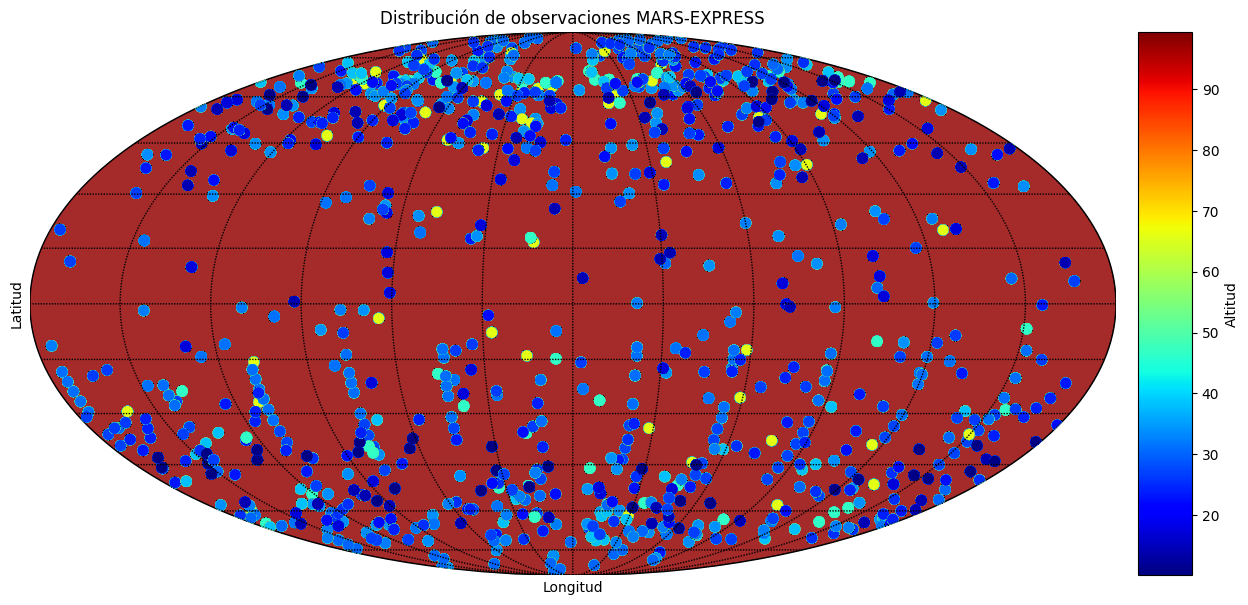
\includegraphics[width=\textwidth, scale=2]{Imagenes/Mars_distrib.png}
    \caption{Distribuci\'on espacial de detecciones de SPICAM [IR] en Marte desde 2004 hasta 2018 para diferentes niveles de altitud.}
    \label{fig:Distrib}
\end{figure*}

Las regiones delimitadas para los primeros resultados de la investigaci\'on en cuesti\'on cubren el \'area superficial marciana entre las coordenadas geogr\'aficas  60$^\circ$ $<$ Lat $<$ 80$^\circ$ y 200$^\circ$ $<$ Lon $<$ 280$^\circ$.\\

Para el caso de la Tierra, la regi\'on cubierta corresponde a un perfil de columna basado en el modelo NRLMSISE 00, en donde los par\'ametros geogr\'aficos de entrada son coordenadas de un punto respecto del cual, el modelo hace la respectiva integraci\'on num\'erica para la determinaci\'on del perfil de columna correspondiente \citep{NRLMSISE_2002, NRLMSISE_2021}, centrado en dicho punto para las dos alturas especificadas, a saber: 55 y 105 km.  As\'i mismo, la distribuci\'on espacial de los datos reducidos es igual para todas las posiciones geogr\'aficas del planeta. 


\section{Resultados}

\subsection{Relación actividad solar y variabilidad atmosférica de Marte}

En la \textbf{Figura~\ref{fig:resultados}} se identifica el margen de variaci\'on de dos curvas de densidad de vapor de H2O en funci\'on de la altura en Marte, para dos fechas caracter\'isticas a un m\'aximo y un m\'inimo solar. Adem\'as, pueden visualizarse las l\'ineas de error correspondientes a los datos, en donde se observa como el error aumenta conforme la detecci\'on se realiza a menor altura de la superficie.

\begin{figure}
\centering
	% To include a figure from a file named example.*
	% Allowable file formats are eps or ps if compiling using latex
	% or pdf, png, jpg if compiling using pdflatex
	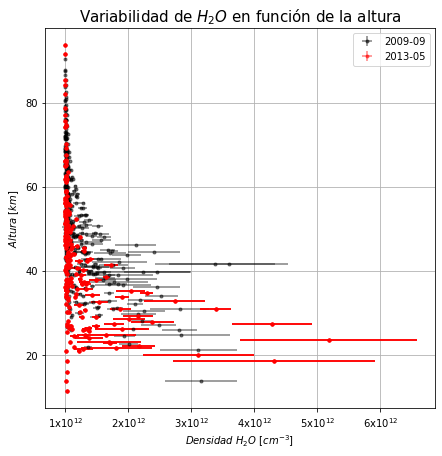
\includegraphics[width=\columnwidth, scale=1]{Imagenes/H2Ovsaltura.png}
    \caption{Variaci\'on de densidad de H$_2$O como funci\'on de la altura para dos fechas características: 05-2013: \'ultimo máximo solar, y 2009-09: \'ultimo m\'inimo solar registrados.  }
    \label{fig:resultados}
\end{figure}


A trav\'es de estos datos y el umbral de resoluci\'on del espectr\'ometro incorporado en SPICAM, se delimita el rango de alturas sobre el cual se establece el an\'alisis en cuesti\'on: entre 30 y 90 km. Para delimitar los tama\~nos de las franjas a estudiar dentro del rango de altura escogido, se tienen en cuenta dos criterios: el primero, la abundancia de datos disponibles a lo largo de los niveles de altura dentro del rango escogido previamente, y el segundo: capas de alturas con espesores por debajo de la altura de escala media del planeta Marte (11.1 km) \citep{Mars_sheet} , garantizando que las variaciones de vapor de H$_2$O en la ventana de tiempo escogida, no se combinen con las variaciones debidas a los cambios de presi\'on de la atm\'osfera a diferentes alturas de la superficie. En este orden de ideas, las franjas escogidas tienen un grosor de 5 km, y los datos que se esbozan en este estudio corresponden a las extensiones verticales de altitud: 50-55 y 70-75 km. Para estas dos franjas de altura, se tienen en promedio 52 detecciones distribuidas de forma desigualmente espaciada, esto dada la frecuencia muestreo del detector de SPICAM y el hecho de que el muestreo ocurre para diferentes latitudes, con diferentes perfiles de alturas dada la velocidad de movimiento orbital de la sonda \textit{Mars Express}. 

Luego se ilustran histogramas de la distribuci\'on de densidades de vapor de agua de la atm\'osfera marciana, en una ventana temporal entre 2004 y 2018 en las dos franjas de altura y posici\'on geogr\'afica seleccionadas como se muestra en los histogramas en las \textbf{Figuras~\ref{fig:hist_M50}} y \textbf{\ref{fig:hist_M70}}. En estos histogramas se delimitan los rangos de variabilidad de vapor de H$_2$O para la ventana temporal en cuesti\'on, respecto de los cuales se lleva a cabo el an\'alisis de relación entre periodo de flujo solar F 10.7 cm y periodo de variabilidad de concentración de H$_2$O en Marte.

\begin{figure}[htp]
	% To include a figure from a file named example.*
	% Allowable file formats are eps or ps if compiling using latex
	% or pdf, png, jpg if compiling using pdflatex
	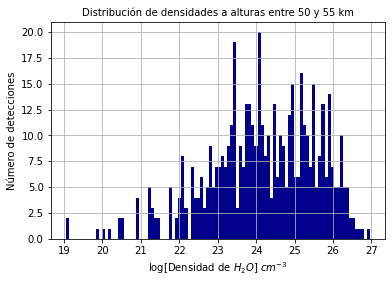
\includegraphics[width=\columnwidth, scale=1]{Imagenes/Hist_M50.png}
    \caption{Histograma distribuci\'on de Densidades de H$_2$O rango de alturas entre 50 y 55 km.}
    \label{fig:hist_M50}
\end{figure}

\begin{figure}[htp]
	% To include a figure from a file named example.*
	% Allowable file formats are eps or ps if compiling using latex
	% or pdf, png, jpg if compiling using pdflatex
	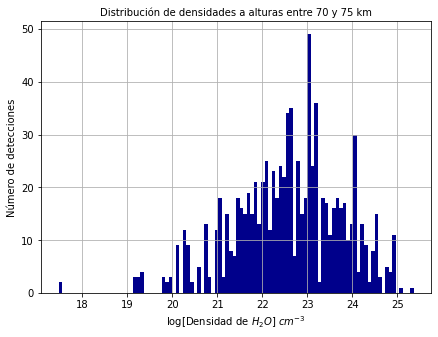
\includegraphics[width=\columnwidth, scale=1]{Imagenes/Hist_M70.png}
    \caption{Histograma distribuci\'on de Densidades de H$_2$O rango de alturas entre 70 y 75 km.}
    \label{fig:hist_M70}
\end{figure}

Con la delimitaci\'on de las regiones a estudiar, se grafica la distribuci\'on de los datos de ambas se\~nales (Flujo solar y densidad de H$_2$O) en la ventana temporal de inter\'es, verificando si en tales distribuciones puede esbozarse alguna relación entre las dos se\~nales (ver \textbf{Figura~\ref{fig:dist_H2O_50y70}}).    


\begin{figure*}
\vspace*{-10mm} %con esta linea se cambia espacio en pagina%
\centering
	% To include a figure from a file named example.*
	% Allowable file formats are eps or ps if compiling using latex
	% or pdf, png, jpg if compiling using pdflatex
	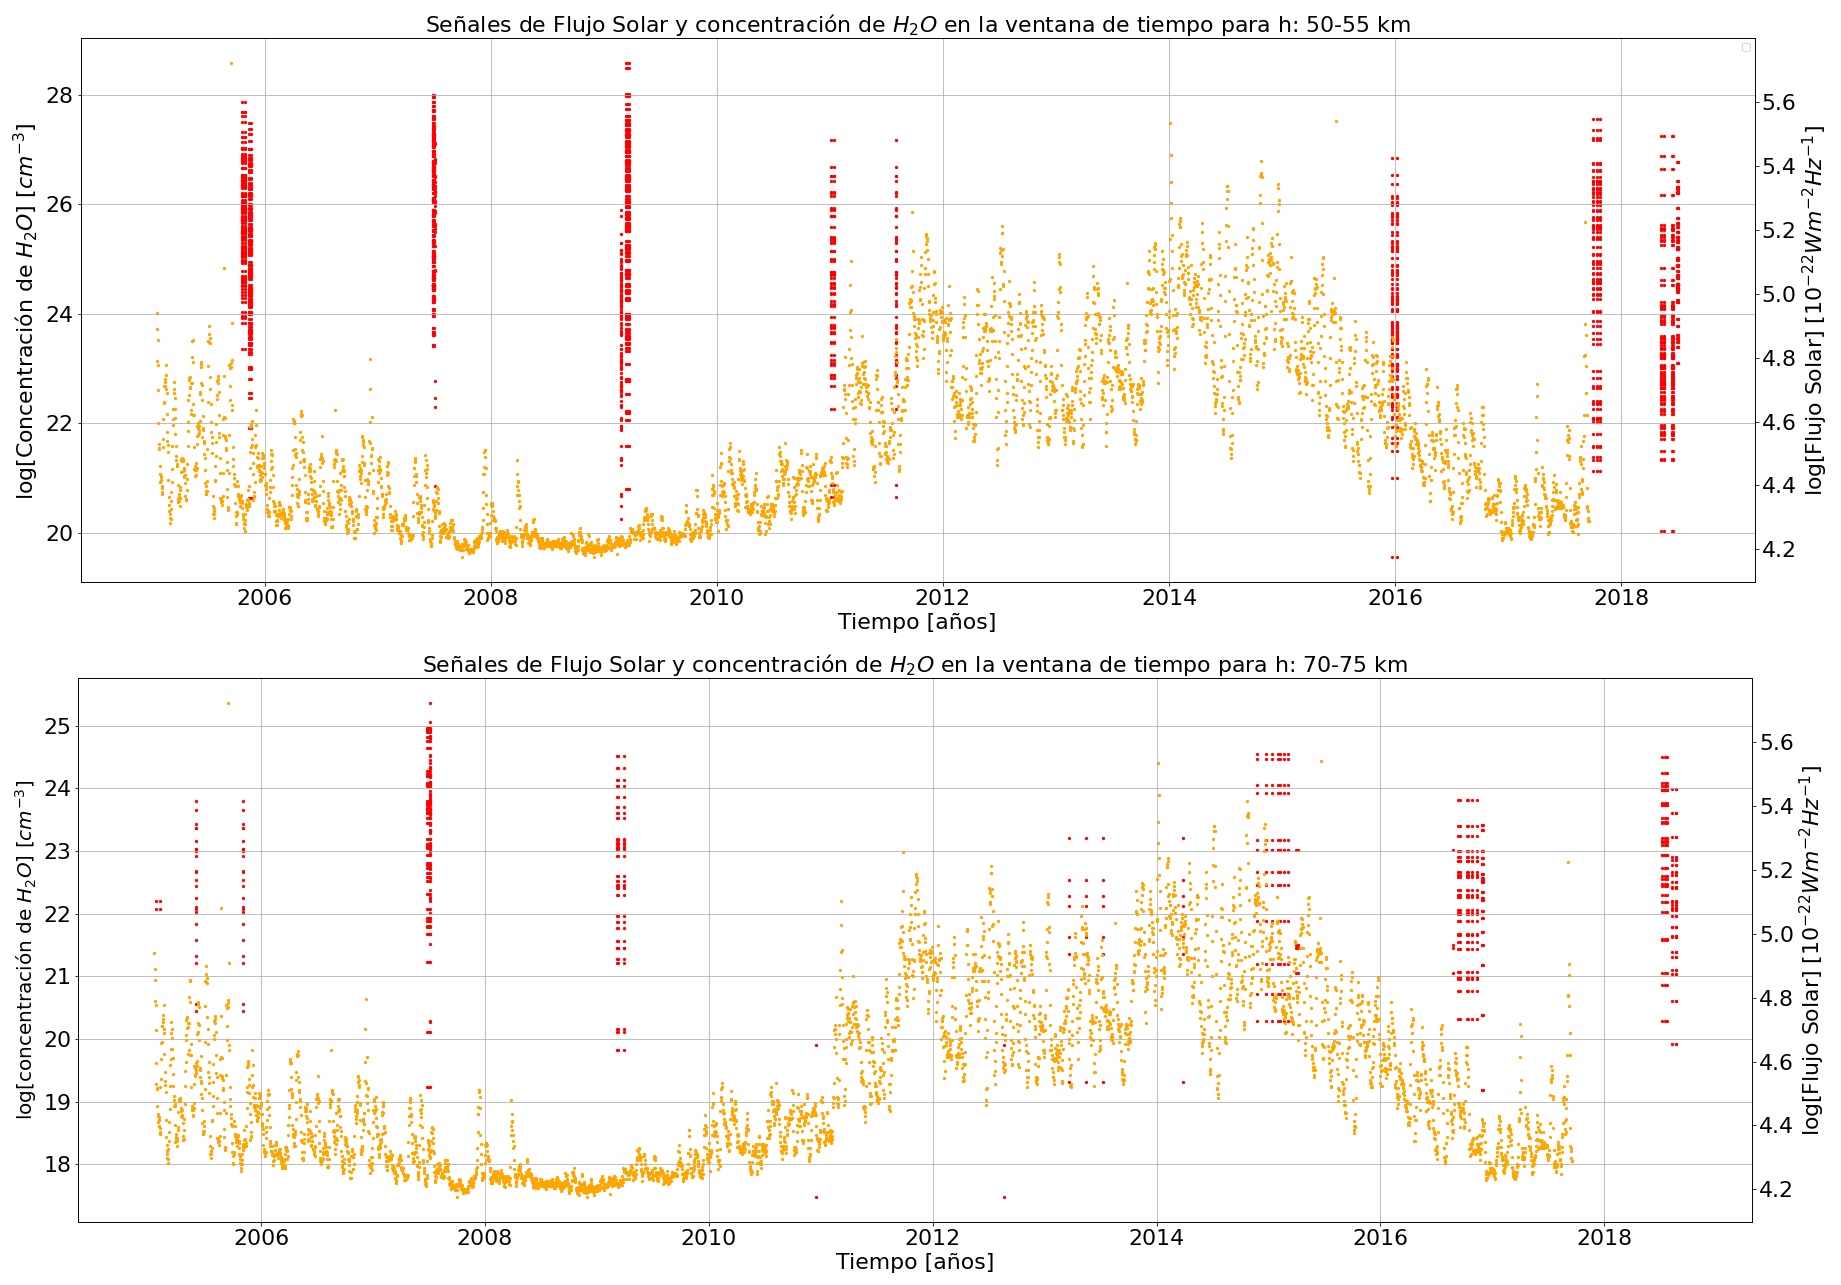
\includegraphics[width=\textwidth, scale=2]{Imagenes/distribucion_H2O_50y70.png}
    \caption{Distribuci\'on temporal de detecciones de H$_2$O SPICAM [IR] en Marte (rojo), en contraste con se\~nal de variaci\'on de flujo solar (naranja) desde 2006 hasta 2018.}
    \label{fig:dist_H2O_50y70}
\end{figure*}


Cuando se tienen calibradas las regiones espaciales sobre las cuales se hace el respectivo an\'alisis de variabilidad y relación entre índice de flujo solar F 10.7 cm y densidad de vapor de H$_2$O, se ajustan los datos de las detecciones de SPICAM de tal modo que se obtienen valores promediados de densidad diaria (desigualmente espaciados), en contraste con valores de flujo solar t\'ipico F 10.7 cm, garantizando la misma resoluci\'on temporal de los dos conjuntos de datos a correlacionar.

El estudio de la relación entre estos dos fenómenos, se lleva a cabo a trav\'es de la caracterizaci\'on peri\'odica de ambas se\~nales, esta caracterizaci\'on se establece mediante la transformaci\'on de la ventana de tiempo al espacio de las frecuencias, de las dos se\~nales a correlacionar, a trav\'es de la transformada r\'apida de Fourier (FFT), en lo que se conoce como el Periodograma de Lomb-Scargle. Este es un m\'etodo que estima el espectro de frecuencias de una se\~nal por medio de un ajuste de m\'inimos cuadrados de funciones arm\'onicas. A diferencia del an\'alisis de Fourier t\'ipico, no se requiere que las observaciones en la ventana de tiempo est\'en igualmente espaciadas \citep{Lomb_1976, scargle_1982}.

Luego de hacer el respectivo an\'alisis de Lomb-Scargle, se esbozan los resultados en el espacio de frecuencias para las se\~nales de flujo solar normalizado logar\'itmicamente y la se\~nal de variaci\'on de vapor de agua igualmente normalizada. Si bien puede observarse la semejanza de las dos se\~nales en algunos picos caracter\'isticos en el espectro de frecuencias, el an\'alisis puede visualizarse con mayor detalle, en tanto se representan los datos en t\'erminos de los periodos asociados a las frecuencias caracter\'isticas de las dos se\~nales para los correspondientes rangos de altura escogidos (ver \textbf{Figuras~\ref{fig:periodogramaLSP_M50}} y \textbf{\ref{fig:periodogramaLSP_M70}}).


\begin{figure}[htp]
	% To include a figure from a file named example.*
	% Allowable file formats are eps or ps if compiling using latex
	% or pdf, png, jpg if compiling using pdflatex
	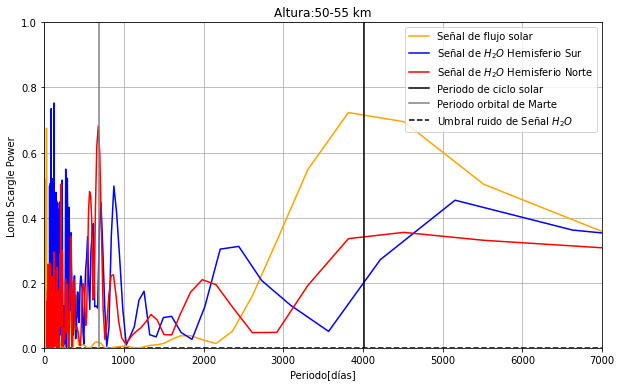
\includegraphics[width=\columnwidth, scale=1]{Imagenes/periodogramaLSP_M50.png}
    \caption{Periodograma de Lomb-Scargle de se\~nales de Flujo Solar y densidad de H$_2$O a la altura 50-55 km, y con marcas temporales de ciclo Solar y periodo orbital de Marte.}
    \label{fig:periodogramaLSP_M50}
\end{figure}

\begin{figure}[htp]
	% To include a figure from a file named example.*
	% Allowable file formats are eps or ps if compiling using latex
	% or pdf, png, jpg if compiling using pdflatex
	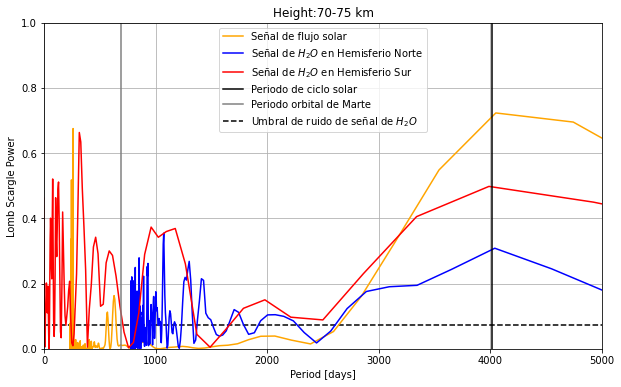
\includegraphics[width=\columnwidth, scale=2]{Imagenes/periodogramaLSP_M.png}
    \caption{Periodograma de Lomb-Scargle de se\~nales de Flujo Solar y densidad de H$_2$O a la altura 70-75 km, y con marcas temporales de ciclo Solar y periodo orbital de Marte.}
    \label{fig:periodogramaLSP_M70}
\end{figure}


\subsection{Correlaciones de especies qu\'imicas en la Tierra}

El modelo emp\'irico NRLMSISE 00 reproduce datos de variabilidad de diferentes especies qu\'imicas a distintas alturas de la atm\'osfera, as\'i como flujo solar caracter\'istico. En las \textbf{Figuras \ref{fig:Time_corr_O2}} y \textbf{\ref{fig:Time_corr_N}} se esbozan las se\~nales de variabilidad de dos especies qu\'imicas (O$_2$ y N) que presentan mayor volatilidad a la altura de 105 km, en contraste y correlaci\'on aparente con la se\~nal de flujo solar en la ventana temporal 1961-2021. Ambas se\~nales obtenidas del modelo en cuesti\'on. 



\begin{figure*}
\vspace*{-5mm} %con esta linea se cambia espacio en pagina%
\centering
	% To include a figure from a file named example.*
	% Allowable file formats are eps or ps if compiling using latex
	% or pdf, png, jpg if compiling using pdflatex
	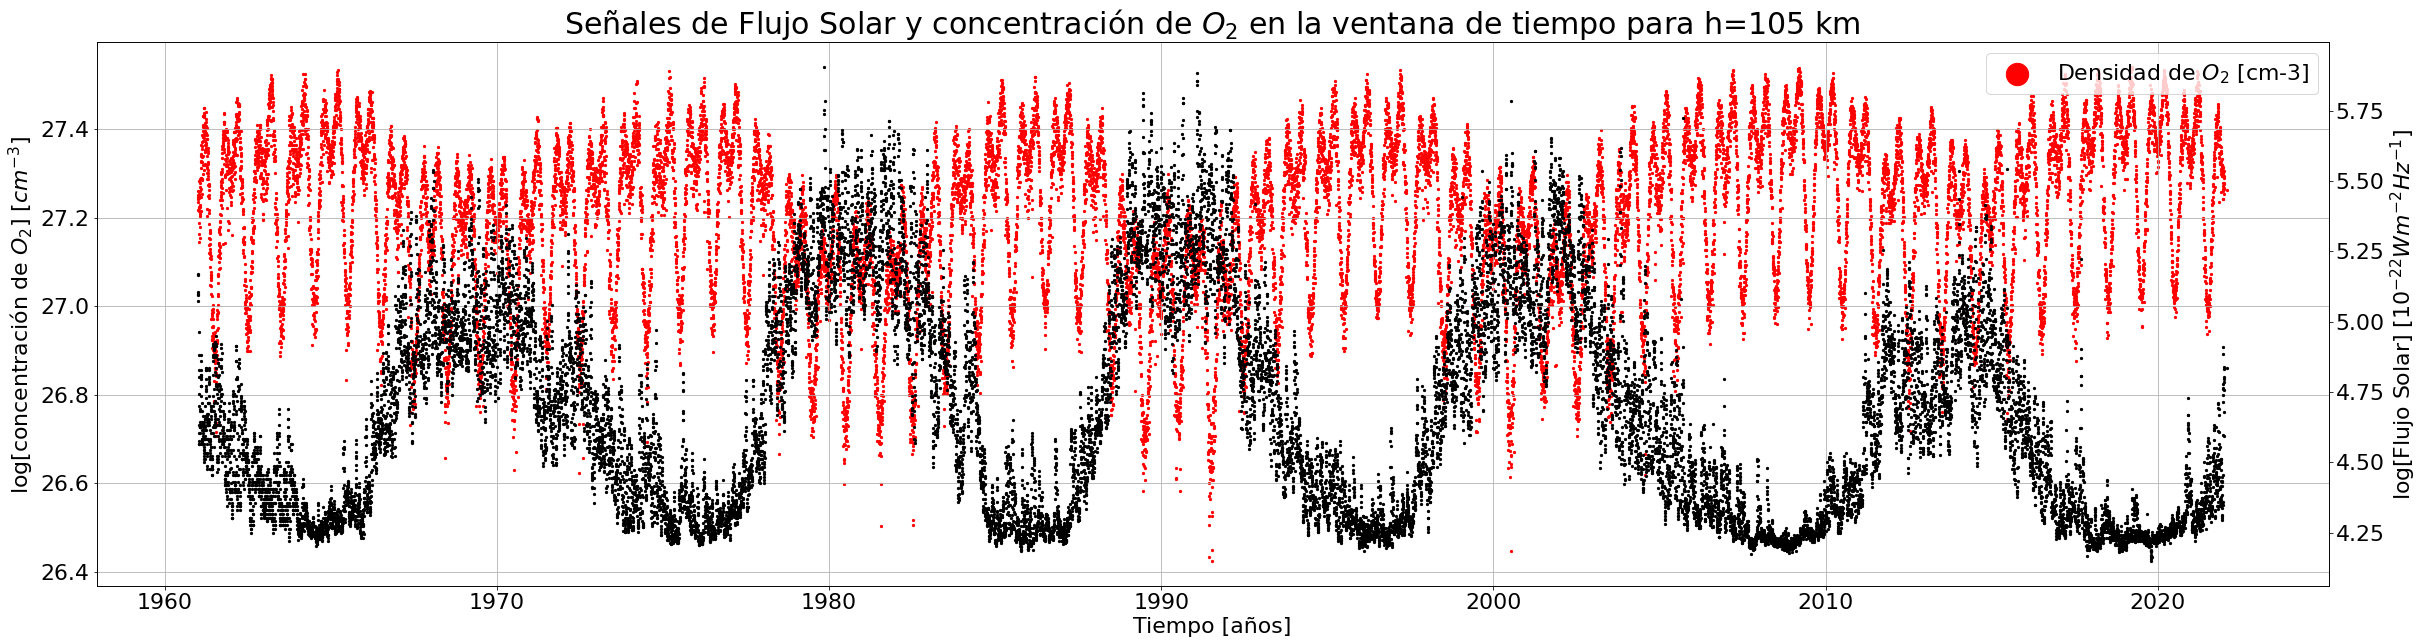
\includegraphics[width=\textwidth, scale=2]{Imagenes/Time_corr_O2.png}
    \caption{Distribuci\'on temporal de $O_2$ en la Tierra a una altura de 105 km, en contraste con se\~nal de variaci\'on de flujo solar en la ventana temporal de 1961-2021.}
    \label{fig:Time_corr_O2}
\end{figure*}

\begin{figure*}
\vspace*{-4mm} %con esta linea se cambia espacio en pagina%
\centering
	% To include a figure from a file named example.*
	% Allowable file formats are eps or ps if compiling using latex
	% or pdf, png, jpg if compiling using pdflatex
	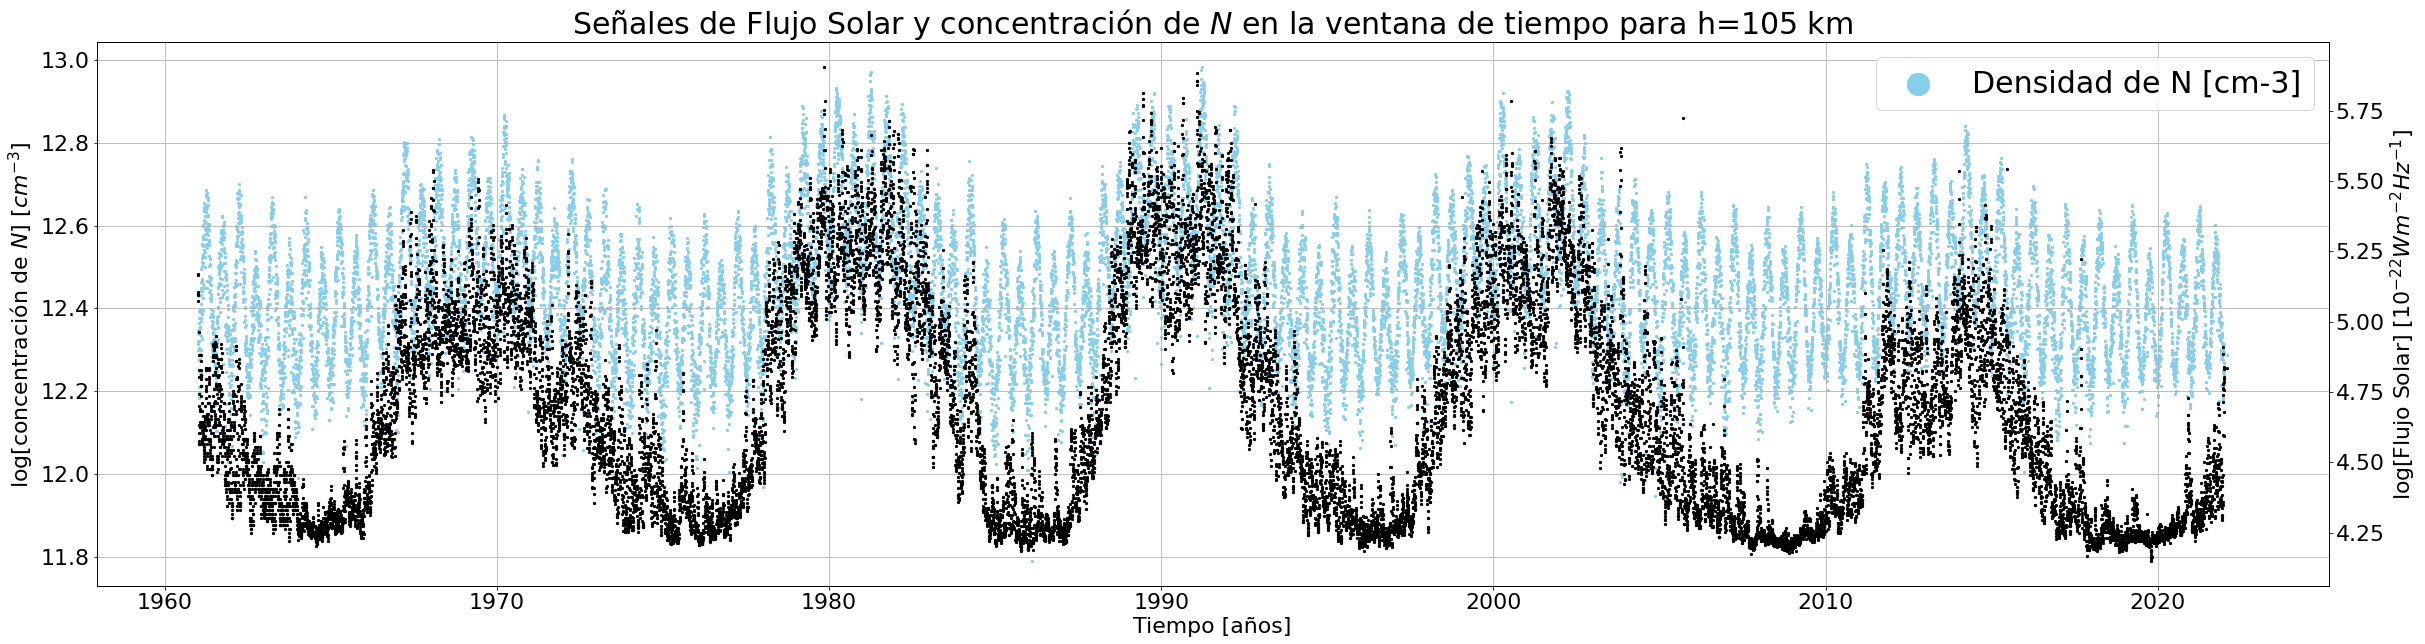
\includegraphics[width=\textwidth, scale=2]{Imagenes/Time_corr_N.png}
    \caption{Distribuci\'on temporal de $N_2$ en la Tierra a una altura de 105 km, en contraste con se\~nal de variaci\'on de flujo solar en la ventana temporal de 1961-2021.}
    \label{fig:Time_corr_N}
\end{figure*}



Los resultados del m\'etodo de Periodograma de Lomb Scargle, para el caso de variaci\'on de densidades de algunas especies qu\'imicas a estudiar en la atm\'osfera de la Tierra, en correspondencia con la se\~nal asociada a la variaci\'on de flujo solar, se esbozan en t\'erminos de los periodos en la \textbf{Figura~\ref{fig:periodogramaLSP_E55}} para una altura de 55 km y en la \textbf{Figura~\ref{fig:periodogramaLSP_E105}} para la altura de 105 km.

\newpage
\begin{figure}[h!]
\vspace{1mm}
	% To include a figure from a file named example.*
	% Allowable file formats are eps or ps if compiling using latex
	% or pdf, png, jpg if compiling using pdflatex
	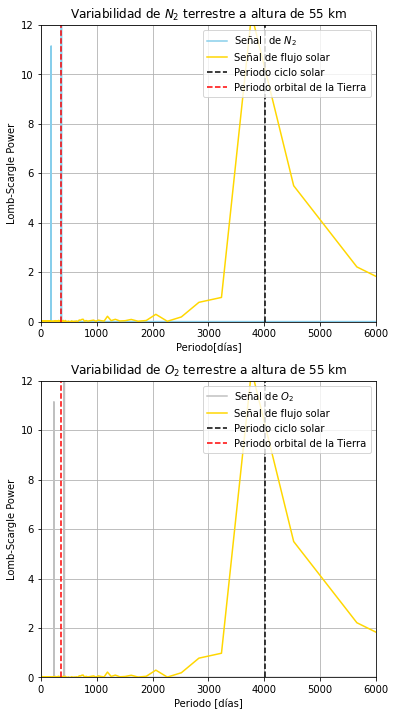
\includegraphics[width=\columnwidth, scale=1]{Imagenes/LSP_Earth55.png}
    \caption{Periodograma de Lomb-Scargle de se\~nales de Flujo Solar y densidad de distintas especies qu\'imicas en la Tierra, a h=55 km. Observe las marcas temporales de ciclo Solar y periodo orbital terrestre.}
    \label{fig:periodogramaLSP_E55}
\end{figure}

\begin{figure}[h!]
	% To include a figure from a file named example.*
	% Allowable file formats are eps or ps if compiling using latex
	% or pdf, png, jpg if compiling using pdflatex
	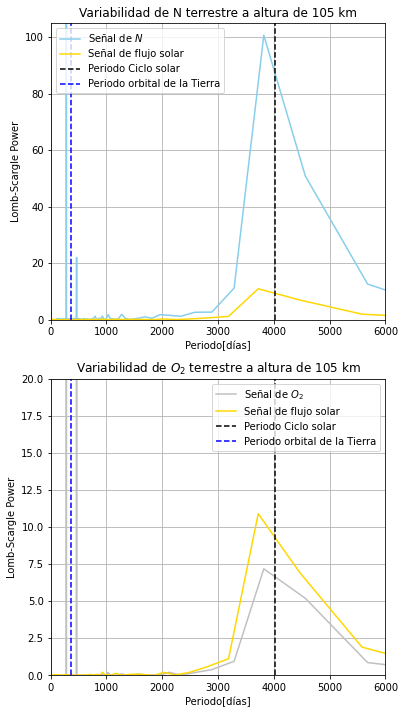
\includegraphics[width=\columnwidth, scale=1]{Imagenes/LSP_Earth105.png}
    \caption{Periodograma de Lomb-Scargle de se\~nales de Flujo Solar y densidad de distintas especies qu\'imicas en la Tierra, a h=105 km. Observe las marcas temporales de ciclo Solar y periodo orbital terrestre.}
    \label{fig:periodogramaLSP_E105}
\end{figure}


Obs\'ervese la diferencia en los picos de las se\~nales asociadas con el periodo del ciclo solar en la Tierra (ver \textbf{Figura~\ref{fig:periodogramaLSP_E105}}), para las alturas m\'as altas, en comparaci\'on con las m\'as bajas, en contraste con los picos de frecuencia y periodos de variabilidad de las se\~nales qu\'imicas.

De acuerdo con el registro de datos del modelo atmosf\'erico NRLMSISE 00, en la zona baja de la atm\'osfera terrestre a 55 km no se registran grados de abundancia de $N$ (Nitrógeno), especie qu\'imica que a la altura de 105 km, manifiesta un comportamiento altamente variable en la ventana de tiempo con una resoluci\'on temporal de 1 d\'ia. El pico de potencia (Potencia Lomb-Scargle) del $N$ en un periodo cercano al del ciclo solar, supera en intensidad al pico correspondiente a la se\~nal de variaci\'on de flujo solar \textbf{(Figura~\ref{fig:periodogramaLSP_E105}}).


\subsection{S\'intesis de resultados variabilidad atmosf\'erica Tierra, Marte y ciclo solar}


En general, para las especies qu\'imicas analizadas con el m\'etodo de Lomb Scargle, a la altura de 105 km (para la Tierra) y el rango de alturas 70-75 km (para Marte), parecen existir correlaciones marcadas con la curva de variabilidad de flujo solar, especialmente en valores peri\'odicos de tiempo cercanos a los 11 a\~nos del ciclo solar, a expensas de las siguientes sutilezas: 

En las se\~nales de variabilidad en la concentraci\'on de agua en la atm\'osfera de Marte, manifiestas en el periodograma de Lomb-Scargle a un rango de altura de 50-55 km de la superficie, se denota semejanza de picos entre la se\~nal de flujo solar y la se\~al de variabilidad de vapor de agua en el hemisferio Norte del planeta. En tanto, la se\~nal de esta misma especie qu\'imica, en hemisferio sur, parece estar levemente desfasada. Este efecto se da tambi\'en para los datos de vapor de H$_2$O en el rango de alturas 70-75 km (\textbf{Figura~\ref{fig:periodogramaLSP_M70}}).

Los desfases podr\'ian estar relacionados con el hecho de que hay dos ciclos de Marte involucrados  en un periodo de variabilidad de actividad solar. El primero, la variación en la concentración de H$_2$O, asociada al periodo de actividad solar (hipótesis del estudio), y el segundo, la variación asociada al periodo orbital estacional. La combinación de estos dos ciclos, y el hecho de que no coincidan el uno con el otro, podría ser la causa de los desfases en los periodogramas respecto del periodo de ciclo solar. El desfase observado en cada uno de los dos hemisferios, también Podr\'ia estar asociado a la variaci\'on estacional que determina los momentos de la \'orbita en que los hemisferios experimentan mayor o menor exposici\'on a la radiaci\'on solar seg\'un grado de inclinaci\'on del eje de rotaci\'on del planeta, que para el caso de Marte es similar al de la Tierra \citep{Mars_sheet}.

La concordancia entre los dos picos de variabilidad de las dos se\~nales emparejadas (flujo solar y especie qu\'imica) en el valor del periodo que corresponde al ciclo solar parece sugerir la existencia de relación entre estas se\~nales para alturas dentro de la termosfera de ambos planetas. Sin embargo, en los resultados preliminares que se esbozan en este estudio, determinar en rigor la existencia de una relación precisa entre ambas se\~nales para distintas especies qu\'imicas, es un trabajo que requiere contrastaci\'on de datos con otros orbitadores, as\'i como llevar a cabo un an\'alisis estad\'istico de correlaci\'on m\'as profundo sobre los datos, que no corresponde a los objetivos de la investigación preliminar que se presenta en esta publicaci\'on.



\section{Conclusiones}

De acuerdo a los resultados obtenidos en el presente trabajo, se encuentra una posible relación entre periodo de variaci\'on de actividad solar, y los cambios en densidad de las especies qu\'imicas escogidas para la Tierra a una altura de 105 km de la superficie. Igualmente, se encuentra con la variaci\'on de actividad solar una variación en la concentraci\'on de vapor de H$_2$O en la termosfera baja de Marte a la luz del m\'etodo aplicado en esta primera fase de la inviestigaci\'on. El panorama de investigación se puede ampliar en futuros trabajos con el estudio a otras especies qu\'imicas en Marte a partir de datos de otras naves de sondeo atmosf\'erico, como \textit{Mars Reconnaissance Orbiter} y MAVEN (\textit{Mars Atmosphere and Volatile Evolution}). 


\section*{Agradecimientos}

JNMC agradece especialmente al Group of Solar Astrophysics (GoSA) y al Observatorio Astronómico Nacional por ser el espacio en donde las diversas retroalimentaciones recibidas dieron buen rumbo a la propuesta.  También se agradece a James R. Murphy  por los consejos en cuanto al procesamiento de los datos de orbitadores antiguos de Marte (\textit{Mars Express} y \textit{Mars Reconnaissance Orbiter} (MRO). Finalmente, un agradecimiento al Colectivo Orbitamautas por ser el espacio informal en donde se pudo poner a prueba la capacidad comunicativa de este trabajo. 



%\section*{Referencias bibliográficas}
%Para incluir la lista de referencias bibliográficas se puede hacer de las dos formas que se indican abajo: ingresando cada referencia con el comando "bibitem" en este documento, o usando un el archivo bibligrafia.bib.
%Para citar una referencia bibliográfica en el texto, se utiliza el comando \verb|\cite{}|. Por ejemplo, si queremos citar un artículo de un autor llamado Scargle publicado en 1982, escribimos \cite{scargle_1982}, que se encuentra en este caso en el listado de artículos dentro del archivo bibliografia.bib.

%Forma 1 de incluir referencias
%\begin{thebibliography}{}
%   \bibitem{smith2005}
 %   Smith, J. (2005). Título del artículo. Nombre de la revista, vol. 1, páginas 1-10.
 %   \bibitem{jones2010}
  %  Jones, A. (2010). Título del libro. Editorial X.
%\end{thebibliography}


%Forma 2 de incluir referencias
\bibliography{biblio}


\end{document}